\subsection{SSC Metalmark}

\begin{center}
    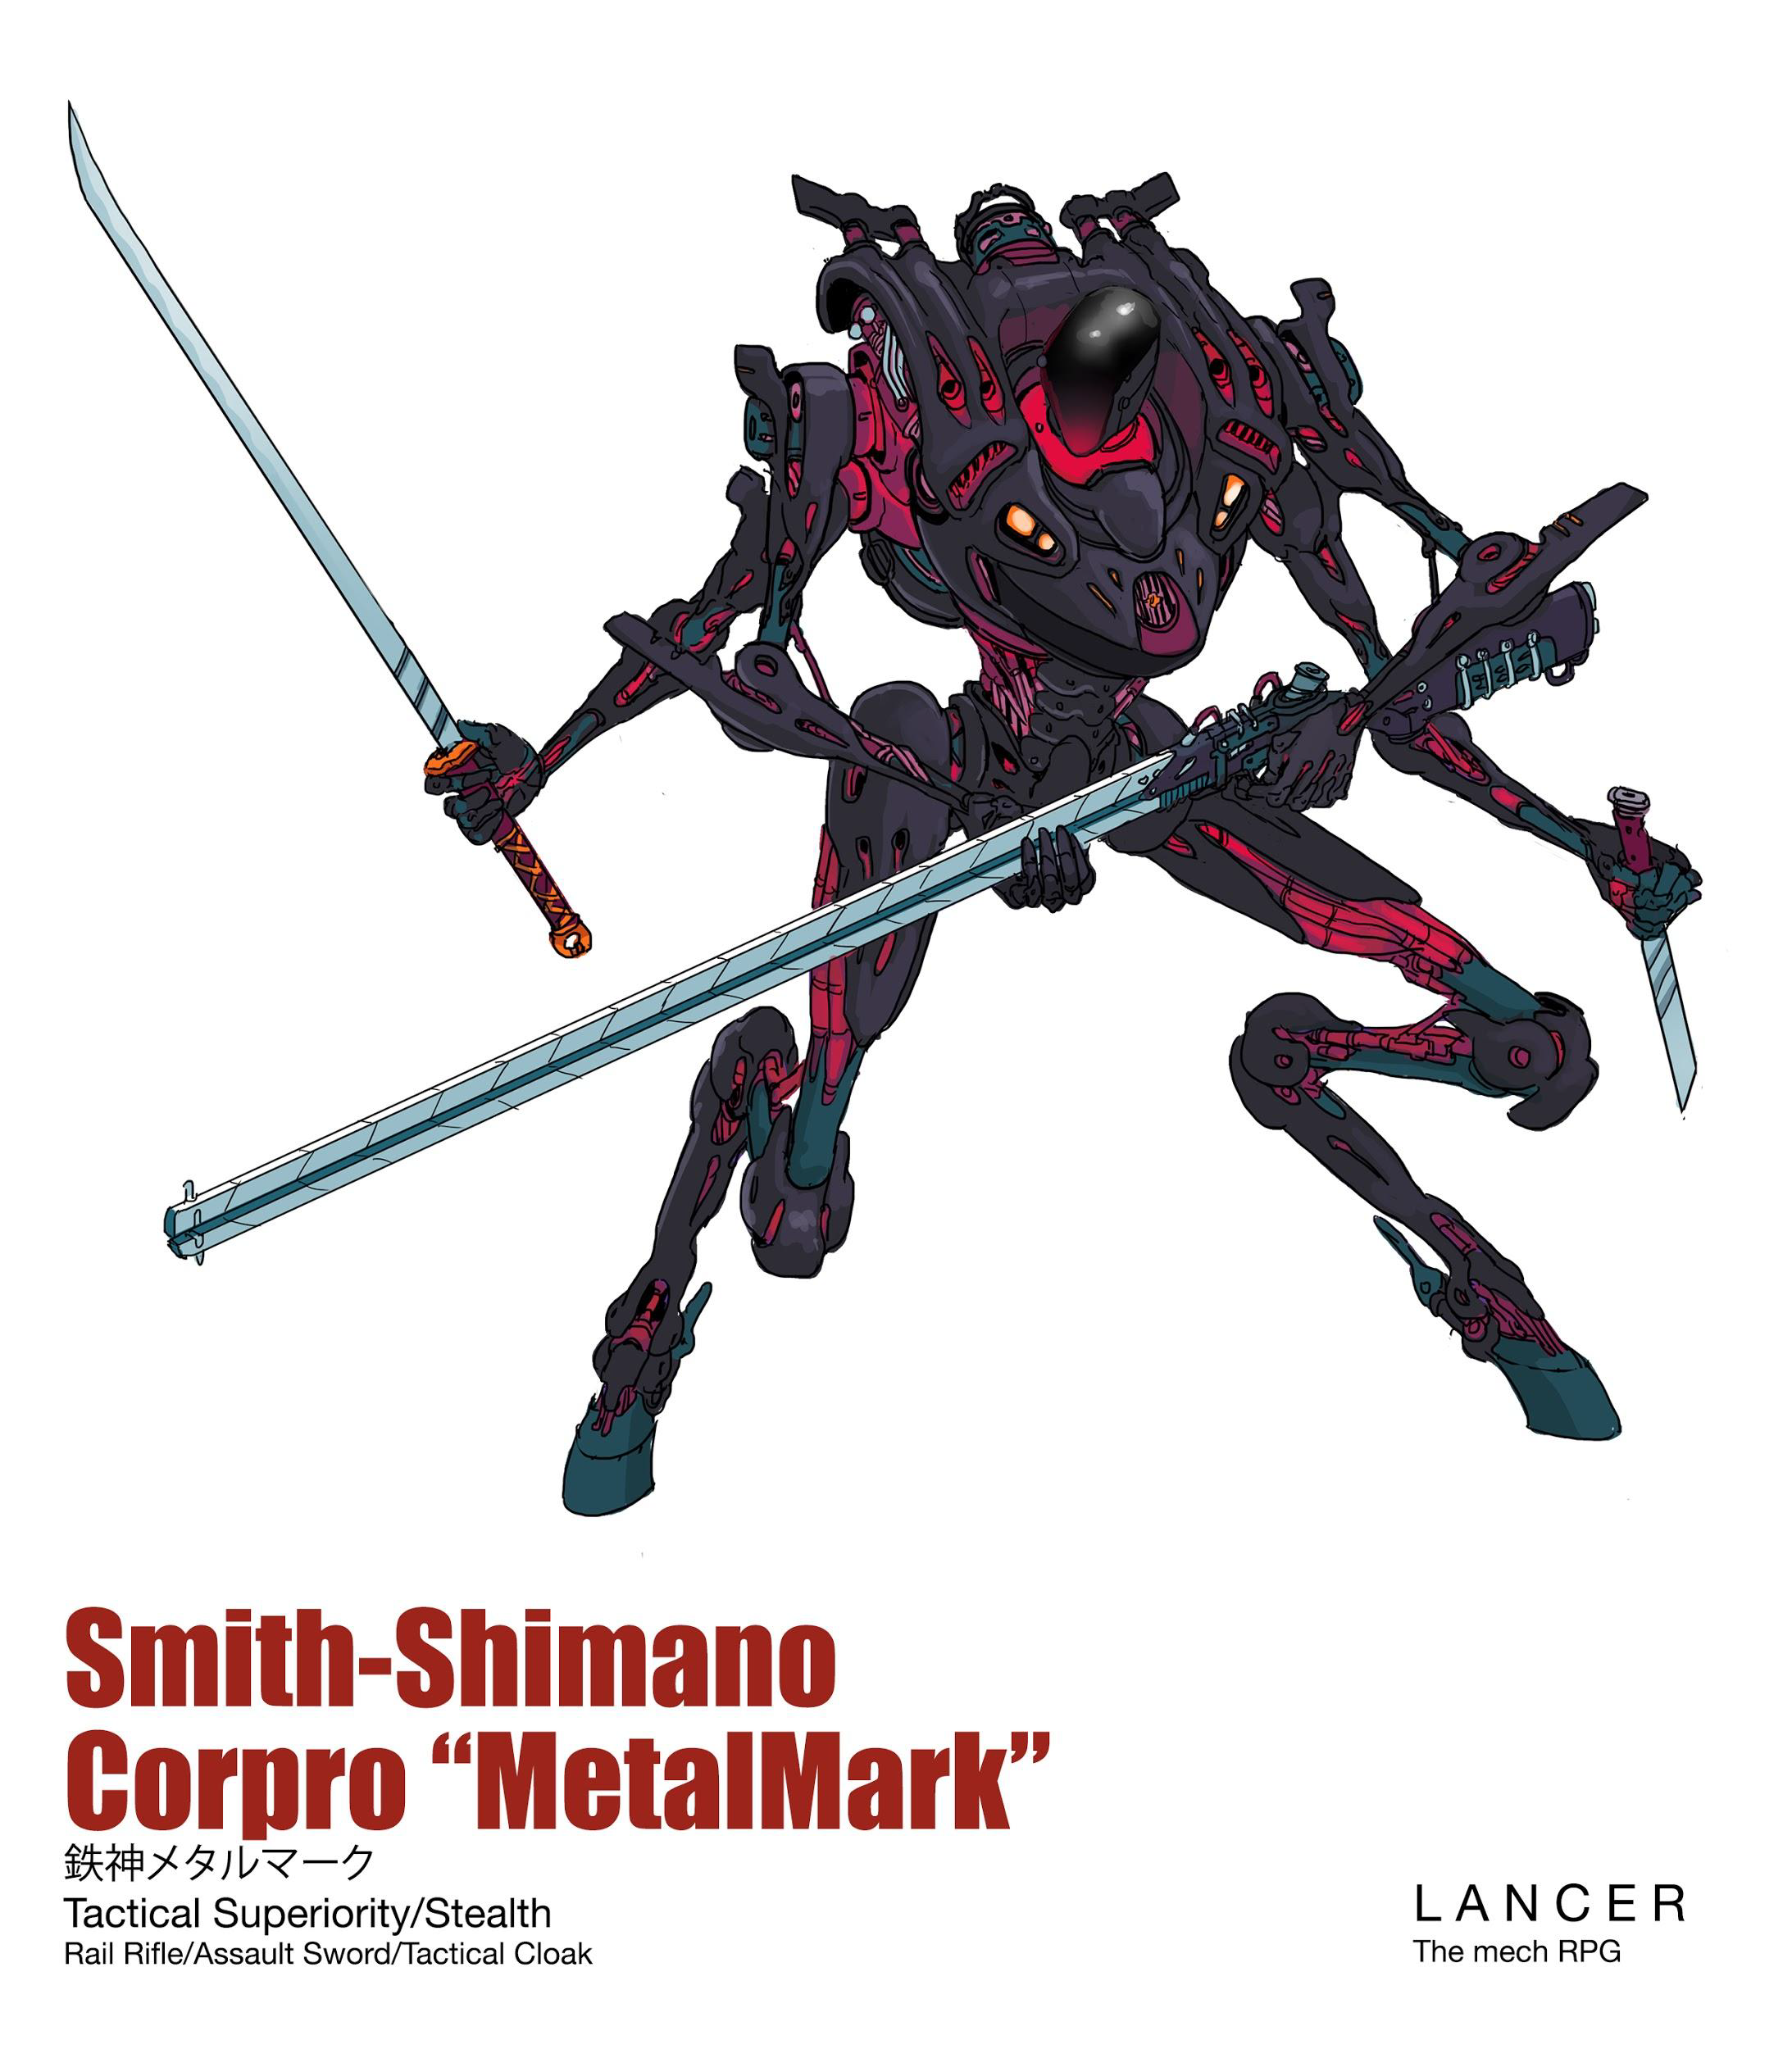
\includegraphics{Metalmark}
\end{center}

\begin{mech}
\fluff{The METALMARK is SCC's backbone-class line mech, fully equipped with SSC's proprietary design and engineering hallmarks to ensure that it is just as survivable as it is agile. The METALMARK base model reflects SSC's deep-space and long patrol heritage in its aquiline design, sturdy construction, and multiple redundant systems. All METALMARK models come standard with a SMITH CUSTOM LEATHER gimbaled pilot seat to ensure comfort on long distance ranging expeditions.}

\begin{license}
\item Flash Grenade, Reactive Weave
\item METALMARK FRAME, Shock Wreath, Rail Rifle
\item Active Camo, Shock Knife
\end{license}

\frameBox
[hp = 8,
evasion = 9,
speed = 5,
heat cap = 5,
sensors = 10,
armor = 1,
e-defense = 8,
size = 1,
repair cap = 4,
tech attack = +0,
traits = {\textbf{Flash Cloak:} The metalmark is invisible while moving (regular move, boosting, moves from talents, etc), but reappears after it finishes its movement.

\textbf{Carapace Adaptation:} When the METALMARK would benefit from light cover, it instead benefits from heavy cover},
sp = 5,
mount one = aux/aux mount,
mount two = main mount,
mount three = heavy mount,
core system name = Tactical Cloak,
core system text = {A tight-knit, tight-bind weave of reactive fabric, tactical cloaks are high-license tech, restricted to pilots of METALMARK classification II or higher. The weave covers roughly 80\% of a chassis, giving it an overall dull quality when viewed through optics or with the naked eye. It is difficult to target, and when activated it bends light in such a way that makes it nearly impossible to see.},
core active name = Cloaking Protocol,
core active text = {Active (Requires 1 core power):Protocol
Until the end of the current challenge, or when you deactivate this module at the start of your turn, you become invisible. If you take damage, you lose the benefit of this module until the start of your next turn. No other action will deactivate it.}]


Reactive Weave

A woven CSAJ (Critical Systems And Joints) cover, Reactive Weave not only protects sensitive systems and joints from fouling and poor weather, but provides a surface for SSC engineers to apply their unique loomware technology. This weave is powered, capable of free-flexing to augment a mech's mobility and reduce the stress placed on a chassis' joints.

1 SP, Unique

When you brace, your mech can immediately move its speed as a reaction and it also gains invisibility until the end of its next turn.


Flash Grenade

2 SP, Limited (2)
Grenade

This grenade can be thrown to a space in range 5. When this grenade explodes, it creates a burst 2 zone that lasts until the end of your next turn. Actors other than you (allied or enemy) caught inside can't trace line of sight out of the zone (they can attack other targets inside normally), and actors inside the zone benefit from light cover.


Shock Wreath

An after-fabrication modification popular among melee-oriented pilots, the Shock Wreath applies an integrated bundle of conductive filaments to the blade, point, tip, or surface of a close combat weapon. Paired with a power source (typically in the hilt or half of a weapon, but sometimes external), the Shock Wreath adds a thermal element to the kinetic, and a distinct visual marker: their weapons are picked out in fine lines of white-hot light, shrouded in heat shimmer.

2 SP
Mod

Choose 1 melee weapon. It gains Burn depending on its size (Aux: Burn 1, Main: Burn 2, Heavy
or larger: Burn 3). If it already has Burn, this increases the burn it deals by the same amount.


Rail Rifle

A rail rifle is a popular weapon for pilots in any theater, but the only choice for those operating in atmospheres made up of highly combustible gasses. Using a line of cascading electromagnets, a rail rifle accelerates a small projectile up to tremendous speeds, launching it without combustion or heat reactions. A rail weapon is kinetic and comparatively quiet when fired next to combustion weapons, though its energy signature is difficult to mask given the massive power requirements demanded by the weapon system.

Main Rifle
1 heat (self), Line 12
1d6 kinetic damage


Active Camo

Active camouflage represents the pinnacle of counter-optic defense systems. By interpreting incoming visible-light spectrum data, an active camouflage system can project a light-bending field around its user, effectively hiding them in plain sight.

3 SP, Unique
2 heat (self), Protocol

You can activate or deactivate the light bending properties of this module at the start of your turn. It lasts until the end of your next turn. While this module is active you are invisible. If you take damage, this module immediately deactivates.


Shock Knife

The shock knife is a mech-sized blade made to accept and integrate the post-fabrication Shock Wreathe system. The knives are custom-fabricated by SSC's Terashima artisan enclave, each one bearing its stamp.

Auxiliary Melee

1 heat (self)
Thrown 5, Threat 1
1 energy damage + Burn 2
\end{mech}
